
\subsection{Low-depth (allele frequencies)}

%%%%%%%%%%%%%%%%%%%%%%%%%%%%%%%%%%%%%%%%%

\begin{frame}
\frametitle{Sample allele frequency likelihoods}

        \begin{equation*}
                        P(D|f) = \prod_{i=1}^N \sum_{g \in \{0,1,2\}} P(D|G=g) P(G=g|f)
        \end{equation*}

	\begin{center}
                \begin{tabular}{| c | c | c | c | c |}
			\hline
			$P(D|f=0)$ & $P(D|f=1)$ & $P(D|f=2)$ & ... & $P(D|f=2k)$\\
			\hline
                \end{tabular}
                with $k$ diploids.
        \end{center}

\end{frame}

%%%%%%%%%%%%%%%%%%%%%%%%%%%%%%%%%%%%%%%%%%

\begin{frame}
\frametitle{Sample allele frequency probabilities}

	\begin{figure}
                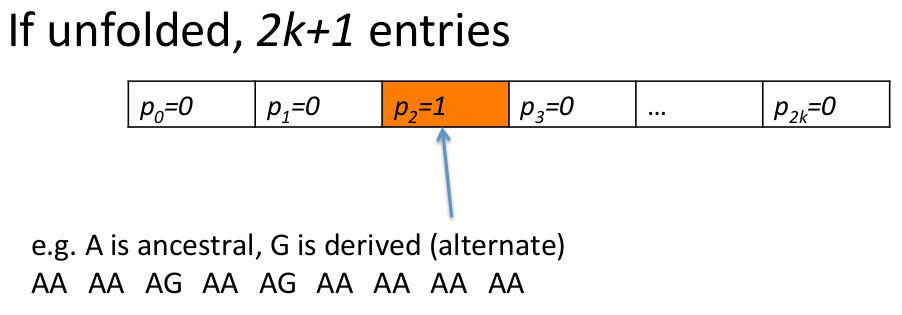
\includegraphics[width=\textwidth]{Pics/saf_1.png}
        \end{figure}
	
	If genotypes are unknown and counting is not possible?

\end{frame}

%%%%%%%%%%%%%%%%%%%%%%%%%%%%%%%%%%%%%%%%%%

\begin{frame}
\frametitle{Sample allele frequency probabilities}

        \begin{figure}
                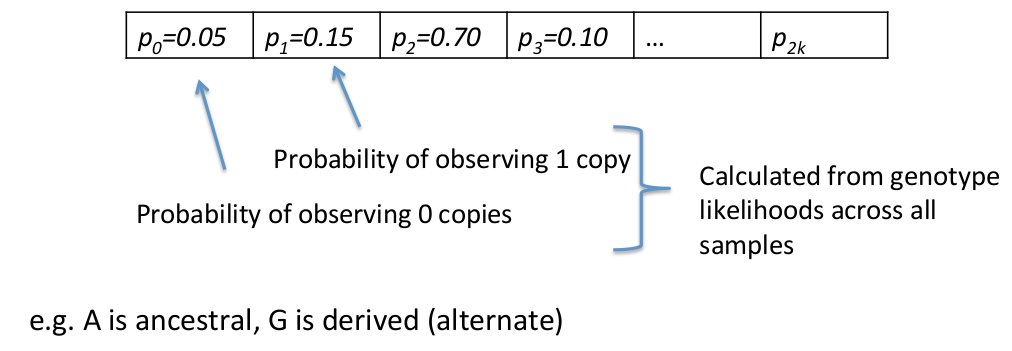
\includegraphics[width=\textwidth]{Pics/saf_2.png}
        \end{figure}

        If genotypes are unknown and counting is not possible.

\end{frame}

%%%%%%%%%%%%%%%%%%%%%%%%%%%%%%%%%%%%%%%

\begin{frame}
\frametitle{Sample allele frequency probabilities}

        \begin{figure}
                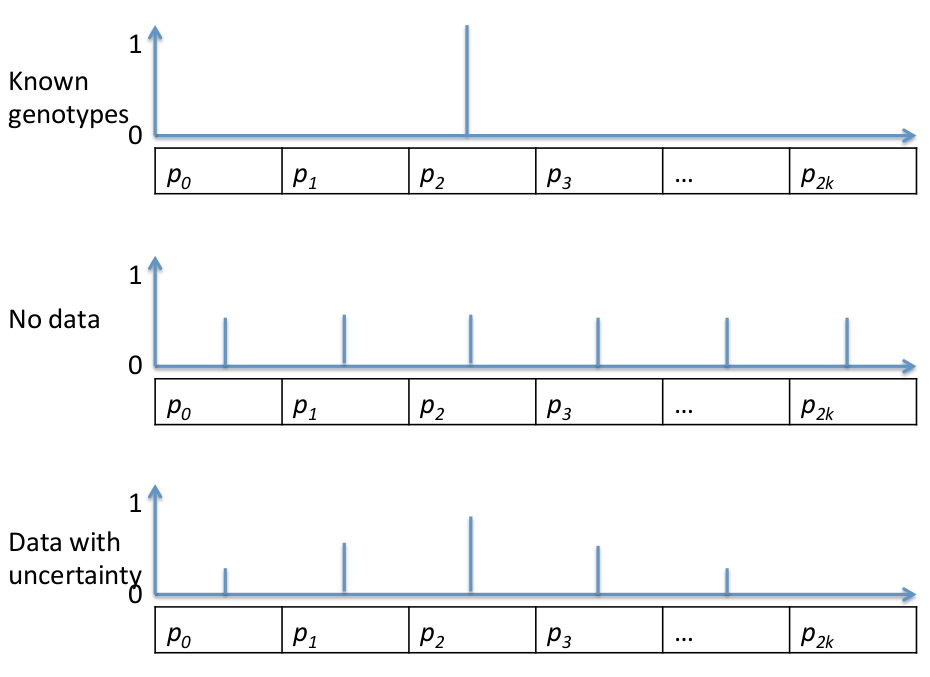
\includegraphics[width=0.7\textwidth]{Pics/saf_3.png}
        \end{figure} 

\end{frame}


%%%%%%%%%%%%%%%%%%%%%%%%%%%%%%%%%%

\begin{frame}
\frametitle{Sample allele frequency probabilities}

	Summary statistics

	\small{
	\begin{center}
                \begin{tabular}{| c | c | c | c | c |}
                        \hline
                        $P(f=0|D)$ & $P(f=1|D)$ & $P(f=2|D)$ & ... & $P(f=2k|D)$\\
                        \hline
                \end{tabular}\\
                with $k$ diploids.
        \end{center}
	}

	\begin{center}
		\Large{
		$\hat{f} = \pause \sum_{i=0}^{2k} (\frac{i}{2k}) \cdot P(f=i|D) $
		}
	\end{center}

\end{frame}

%%%%%%%%%%%%%%%%%%%%%%%%%%%%%%%%

\begin{frame}
\frametitle{Sample allele frequency probabilities}

        Summary statistics

        \small{
        \begin{center}
                \begin{tabular}{| c | c | c | c | c |}
                        \hline
                        $P(f=0|D)$ & $P(f=1|D)$ & $P(f=2|D)$ & ... & $P(f=2k|D)$\\
                        \hline
                \end{tabular}\\
                with $k$ diploids.
        \end{center}
        }

        \begin{center}
                \Large{
                $P_{\textit{var}} = \pause 1 - P(f=0|D) - P(f=2k|D) $
                }
        \end{center}

\end{frame}


%%%%%%%%%%%%%%%%%%%%%%%%%%%%%%%%

\begin{frame}
\frametitle{Sample allele frequency probabilities}

        Summary statistics - number of segregating sites

        \small{
        \begin{center}
                \begin{tabular}{| c | c | c | c | c | c |}
                        \hline
                        site 1 & $P(f=0|D)$ & $P(f=1|D)$ & $P(f=2|D)$ & ... & $P(f=2k|D)$\\
			site 2 & $P(f=0|D)$ & $P(f=1|D)$ & $P(f=2|D)$ & ... & $P(f=2k|D)$\\
			site 3 & $P(f=0|D)$ & $P(f=1|D)$ & $P(f=2|D)$ & ... & $P(f=2k|D)$\\
			... & ... & ... & ... & ...\\
			site M & $P(f=0|D)$ & $P(f=1|D)$ & $P(f=2|D)$ & ... & $P(f=2k|D)$\\
                        \hline
                \end{tabular}
        \end{center}
        }

        \begin{center}
                \Large{
                $E[S] = \pause \sum_{j=1}^M \pause (1 - P(f_j=0|D) - P(f_j=2k|D)) $   
                }
        \end{center}

\end{frame}

%%%%%%%%%%%%%%%%%%%%%%%%%%%%%%%%

\begin{frame}
\frametitle{Sample allele frequency probabilities}

        Summary statistics - nucleotide diversity $D=2 \cdot f \cdot (1-f)$

        \small{
        \begin{center} 
                \begin{tabular}{| c | c | c | c | c | c |}
                        \hline
                        site 1 & $P(f=0|D)$ & $P(f=1|D)$ & $P(f=2|D)$ & ... & $P(f=2k|D)$\\
                        site 2 & $P(f=0|D)$ & $P(f=1|D)$ & $P(f=2|D)$ & ... & $P(f=2k|D)$\\
                        site 3 & $P(f=0|D)$ & $P(f=1|D)$ & $P(f=2|D)$ & ... & $P(f=2k|D)$\\
                        ... & ... & ... & ... & ...\\
                        site M & $P(f=0|D)$ & $P(f=1|D)$ & $P(f=2|D)$ & ... & $P(f=2k|D)$\\
                        \hline  
                \end{tabular}
        \end{center}
        }

        \begin{center}
                \Large{
                $E[D] = \pause \sum_{j=1}^M \sum_{i=0}^{2k}  (\frac{i}{2k}) \cdot (\frac{2k-i}{2k}) \cdot P(f_j=i|D) $
                }
        \end{center}

\end{frame}

%%%%%%%%%%%%%%%%%%%%%%%%%%%%%%
\begin{frame}
\frametitle{Site frequency spectrum (SFS)}

	The SFS is a summary of population genetic data.

	Each bin represents the proportion of sites with a particular derived (or minor) allele frequency.

	\begin{figure}
                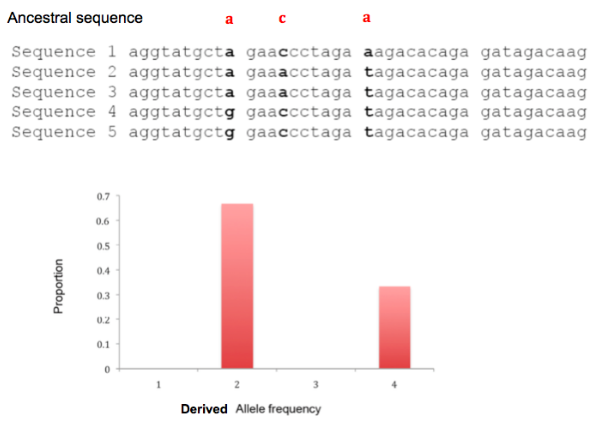
\includegraphics[width=0.7\textwidth]{Pics/sfs_count.png}
        \end{figure}

\end{frame}

%%%%%%%%%%%%%%%%%%%%%%%%%%%%%%%
\begin{frame}
\frametitle{Site frequency spectrum (SFS)}

	SFS under the neutral coalescent model for a sample of $n=11$ haploid individuals.

	\begin{figure}
                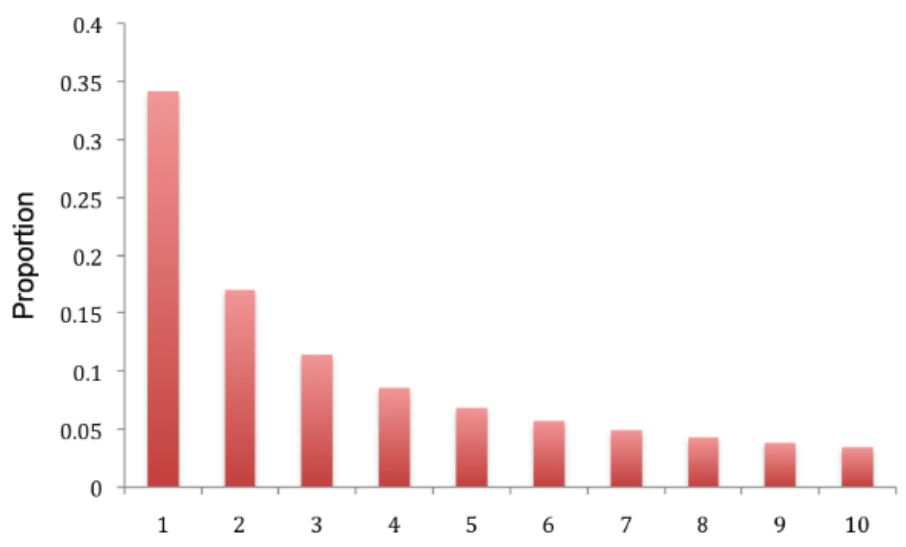
\includegraphics[width=0.7\textwidth]{Pics/sfs_exp.png}
        \end{figure}


\end{frame}

%%%%%%%%%%%%%%%%%%%%%%%%%%%%%%%
\begin{frame}
\frametitle{Site frequency spectrum (SFS)}

	From low-depth data:

        \begin{figure}
                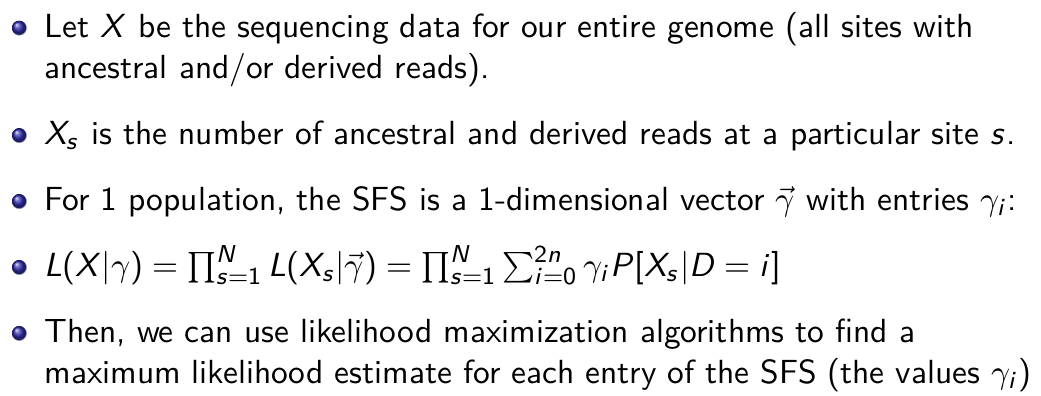
\includegraphics[width=\textwidth]{Pics/sfs_low.png}
        \end{figure}


\end{frame}

%%%%%%%%%%%%%%%%%%%%%%%%%%%%%%%

\begin{frame}
\frametitle{Exercise - 4}

	Calculate the SFS for each population and compare them.

	Estimate summary statistics (e.g. $\pi$, $\theta_W$) and make some comments on their different values.

	Advanced:
	
	Calculate the joint (2D) SFS and $F_{ST}$ in sliding windows.

\end{frame}


